\documentclass[tikz,border=10pt]{standalone}
\usepackage{amsmath}
\usetikzlibrary{arrows.meta, positioning, calc, fit, decorations.pathreplacing}

\definecolor{c1}{HTML}{000000}
\definecolor{c2}{HTML}{233D4D}
\definecolor{c3}{HTML}{FE7F2D}
\definecolor{c4}{HTML}{EAECF0}
\definecolor{axiscolor}{HTML}{333333}
\definecolor{labelcolor}{HTML}{5F6B75}

\begin{document}
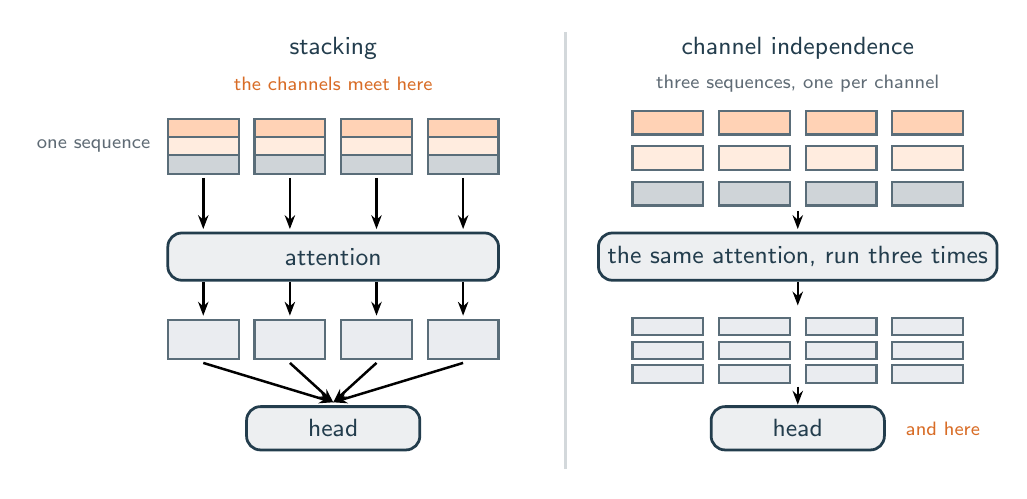
\begin{tikzpicture}[
    every node/.style={font=\sffamily},
    arr/.style={-{Stealth[length=5pt]}, line width=0.9pt, color=c1},
    lab/.style={font=\sffamily\scriptsize, text=labelcolor},
    tag/.style={font=\sffamily\scriptsize, text=c2},
    hot/.style={font=\sffamily\scriptsize, text=c3!85!black},
    box/.style={rectangle, draw=c2!75, line width=0.8pt},
    proc/.style={
        rectangle, rounded corners=5pt, draw=c2, fill=c2!8, text=c2,
        line width=1.0pt, align=center, font=\sffamily\small,
    },
]

% ================================================================ titles
\node[tag, font=\sffamily\small] at (2.75, 6.55) {stacking};
\node[tag, font=\sffamily\small] at (8.65, 6.55) {channel independence};
\draw[c2!20, line width=0.8pt] (5.70, 1.20) -- (5.70, 6.75);

% ================================================================ left: one striped sequence
\node[hot] at (2.75, 6.10) {the channels meet here};
\foreach \x in {0.65, 1.75, 2.85, 3.95}{
    \filldraw[box, fill=c3!35] (\x, 5.418) rectangle (\x+0.90, 5.65);
    \filldraw[box, fill=c3!15] (\x, 5.186) rectangle (\x+0.90, 5.418);
    \filldraw[box, fill=c2!22] (\x, 4.954) rectangle (\x+0.90, 5.186);
    \draw[arr] (\x+0.45, 4.90) -- (\x+0.45, 4.25);
}
\node[lab, anchor=north, align=center] at (2.75, 4.88) {};
\node[lab, anchor=east] at (0.55, 5.30) {one sequence};

\node[proc, minimum width=4.2cm, minimum height=0.60cm] at (2.75, 3.90)
    {attention};

\foreach \x in {0.65, 1.75, 2.85, 3.95}{
    \draw[arr] (\x+0.45, 3.58) -- (\x+0.45, 3.15);
    \filldraw[box, fill=c4] (\x, 2.60) rectangle (\x+0.90, 3.10);
}
\foreach \x in {1.10, 2.20, 3.30, 4.40}{
    \draw[arr] (\x, 2.55) -- (2.75, 2.05);
}
\node[proc, minimum width=2.2cm, minimum height=0.55cm] at (2.75, 1.72) {head};

% ================================================================ right: three separate sequences
\foreach \y/\f in {5.45/{c3!35}, 5.00/{c3!15}, 4.55/{c2!22}}{
    \foreach \x in {6.55, 7.65, 8.75, 9.85}{
        \filldraw[box, fill=\f] (\x, \y) rectangle (\x+0.90, \y+0.30);
    }
}
\node[lab] at (8.65, 6.10) {three sequences, one per channel};

\draw[arr] (8.65, 4.48) -- (8.65, 4.25);
\node[proc, minimum width=4.2cm, minimum height=0.60cm] at (8.65, 3.90)
    {the same attention, run three times};

\draw[arr] (8.65, 3.58) -- (8.65, 3.28);
\foreach \y in {2.90, 2.60, 2.30}{
    \foreach \x in {6.55, 7.65, 8.75, 9.85}{
        \filldraw[box, fill=c4] (\x, \y) rectangle (\x+0.90, \y+0.22);
    }
}
\draw[arr] (8.65, 2.25) -- (8.65, 2.02);
\node[proc, minimum width=2.2cm, minimum height=0.55cm] at (8.65, 1.72) {head};
\node[hot, anchor=west] at (9.90, 1.72) {and here};

\end{tikzpicture}
\end{document}
